\subsection{実験2 ジェスチャー分類問題における入力速度変化に対するモデル精度評価}
提案手法をジェスチャー動画分類問題に適用し, 未学習の入力速度に対するモデル精度評価を行う.

\subsubsection{データセット}
ジェスチャー動画のデータセットとして, SNNの評価で広く用いられる\cite{massa2020efficient}DVSGesture\cite{dvsgesture}を使用した.
DVSGestureはイベントベースビジョンセンサ (DVS128 : \figref{fig:dvs128}) で記録されている.
このセンサでは各ピクセルの輝度変化を非同期に捉え, その変化をイベント$\epsilon$として記録する (\eqrefc{eq:dvs:event}).
\begin{equation}
    \epsilon = (x, y, t, p) \label{eq:dvs:event}
\end{equation}
ここで, $(x, y)$はピクセルの座標, $t$はイベントが発生した時刻である.
また, $p$はイベント強度を表し, ピクセルの輝度変化が正であれば1, 負であれば-1の値を持つ.

イベントベースビジョンセンサによるジェスチャー記録の様子を\figref{fig:dvs:recordview}に示す.
上段が通常のフレームベースカメラで記録したもの, 下段がイベントベースビジョンセンサで記録したものである.
また, 黒色は値が0であることを表し, 青色, 桃色はそれぞれ$p=1, p=-1$のイベントを表す.
イベントは時間的なピクセルの輝度変化を検出するため, ジェスチャーでは動きの多い腕周りのピクセル情報が多く記録される.
% 画像引用元
% https://docs.inivation.com/_static/hardware_guides/dvs128.pdf
\begin{figure}[htbp]
    \centering
    \includesvg[width=0.5\textwidth, inkscapelatex=false]{Static/chap2_sec3_dvs128}
    \caption{DVS128\cite{dvs128fig}}
    \label{fig:dvs128}
\end{figure}

\begin{figure}[htbp]
    \centering
    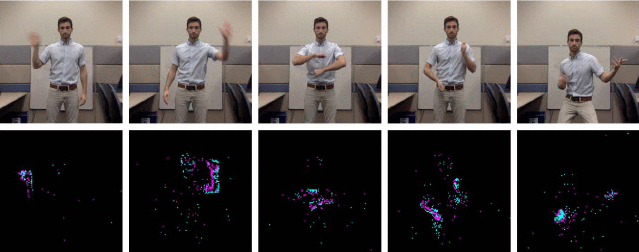
\includegraphics[width=1.0\textwidth]{Static/chap2_sec3_dvs_recordview.png}
    \caption{DVSGesture記録の様子\cite{dvsgesture}}
    \label{fig:dvs:recordview}
\end{figure}

DVSGestureは11種類のクラスのジェスチャーを記録している.
それぞれのジェスチャーのスナップショットを\figref{fig:dvs:gesture}に示す.
\begin{figure}[htbp]
    \centering
    \includesvg[width=0.5\textwidth, inkscapelatex=false]{dummy/dummy_img}
    \caption{各ジェスチャーのスナップショット}
    \label{fig:dvs:gesture}
\end{figure}


\subsubsection{モデルの学習}
モデルの学習はイベントの時系列データを入力, ジェスチャーのクラスを出力とする分類問題として行う.
ここで, 使用するデータセットのイベントの有無をスパイクとして扱うことでSNNの入力としている.
学習させるモデルは, 通常のSNN, Parametric-SNN, 提案手法のSNNとした.
Parametric-SNNとは, ニューラルネットワークの重みとバイアスに加えて, SNNのLIFモデルにおける時定数も学習可能としたSNNである.
モデル構成と学習時のパラメータを\tabref{tab:exp2:model}, \tabref{tab:exp2:model:parameter:lif}, \tabref{tab:exp2:train:parameter}に示す.
また, 学習させたそれぞれのモデル構成は統一で\tabref{tab:exp2:model}のものを用いており, その相違点はニューラルネットワークのバイアスと時定数の学習についてのみである (\tabref{tab:exp2:parameter}).
\begin{table}[htbp]
    \centering
    \caption{ジェスチャー分類モデル構成}
    \label{tab:exp2:model}
    \begin{tabular}{ccccc}
        \hline
        \textbf{Layer}& \textbf{Type}&\textbf{Input size} & \textbf{Output size} & \textbf{Residual block nums}\\
        \hline
        1   & MS-ResNet & 2x32x32 & 12x32x32 & 3\\
        2 & AveragePooling2d & 12x32x32 & 12x16x16 & - \\
        3 & MS-ResNet & 12x16x16 & 32x16x16 & 3\\
        4 & AveragePooling2d & 32x16x16 & 32x8x8 & - \\
        5 & Linear & 2048 & 512 & - \\
        6 & Linear & 512 & 11 & - \\
        \hline
    \end{tabular}
\end{table}

\begin{table}[htbp]
    \centering
    \caption{LIFモデルのパラメータ}
    \label{tab:exp2:model:parameter:lif}
    \begin{tabular}{ccccc}
        \hline
        $\bm{dt}$& $\bm{v_{rest}}$ & $\bm{v_{th}}$ & $\bm{\tau}$ & $\bm{r}$\\
        \hline
        0.003   & 0.0 & 0.1 & 0.006 & 1 \\
        \hline
    \end{tabular}
\end{table}


\begin{table}[htbp]
    \centering
    \caption{モデルの学習条件}
    \label{tab:exp2:train:parameter}
    \begin{tabular}{cc}
        \hline
        学習率 $lr$ & 0.0008\\
        バッチサイズ $batch\_size$ & 64\\
        エポック数 $epoches$ & 800\\
        weight decay $wd$ & 0.001\\
        勾配クリッピング $clip\_norm$ & 1.0\\
        optimizer & AdamW\\
        \hline
    \end{tabular}
\end{table}


\begin{table}[htbp]
    \centering
    \caption{各モデルの相違点}
    \label{tab:exp2:parameter}
    \begin{tabular}{ccccc}
        \hline
         & \textbf{SNN} & \textbf{Parametric-SNN} & \textbf{提案手法}\\
         \textbf{NNのバイアス$b$}&あり&あり&なし($=0$)\\
         \textbf{時定数の学習$\tau$}&なし&あり&あり\\
        \hline
    \end{tabular}
\end{table}

学習時の損失関数を\eqrefc{eq:exp2:loss}に示す.
\begin{align}
    \hat{y}_i &= \frac{1}{T} \sum_{t=1}^T o_i^t \notag \\
    \mathcal{L}_{CE} &= -\sum_{i=1}^{11} y_i \log(\hat{y}_i) \label{eq:exp2:loss}
\end{align}
ここで, $\mathcal{L}_{CE}$はクロスエントロピー損失, $y_i$はone-hotベクトル化した正解ラベルである.
また, SNNの出力$o_i^t$は時間軸を持つため, 単位時間あたりのスパイク密度を$\hat{y}_i$とし, その値をモデルのクラス推論確率としている.
推論時は$\hat{y}_i$が最大のクラスを推論結果とする決定的推論を行う (\eqrefc{eq:exp2:inference}).
\begin{equation}
\hat{y} = \mathop{\arg\max}_{i}(\hat{y}_i) \label{eq:exp2:inference}
\end{equation}



\subsubsection{評価方法}
提案手法の入力速度変化に対する頑健性を評価するために以下の2つの評価を行った.
\begin{itemize}
    \item 入力シーケンス全体を$a$倍速した際のモデル精度評価
    \item 入力シーケンスの前半, 後半をそれぞれ$a_1, a_2$倍速した際のモデル精度評価
\end{itemize}
まず, 入力シーケンス全体の速度倍率を変更したときのモデル精度を評価した.
速度倍率$a$は0.1, 0.2, 0.3, 0.4, 0.5, 0.6, 0.7, 0.8, 0.9, 1.0, 2.0, 3.0, 4.0, 5.0, 6.0, 7.0, 8.0, 9.0, 10.0の20種類の値を用いた.
次に, 入力シーケンスを前半と後半に分割し, 途中で速度倍率を変更した.
このデータを入力したときのモデル精度比較することで, 途中で速度が変更される場合のモデル精度を評価した.
$a_1, a_2$はそれぞれ\tabref{tab:model:parameter:speed:change}に示す値を用いた.
ここで, $a=1.0$は学習時の速度データである.

\begin{table}[htbp]
    \centering
    \caption{速度変更のパラメータ $a_1, a_2$}
    \label{tab:model:parameter:speed:change}
    \begin{tabular}{ccc}
        \hline
        \textbf{Case}& $a_1$ & $a_2$\\
        \hline
        A&1.0&3.0\\
        B&1.0&0.2\\
        C&3.0&0.2\\
        D&0.2&3.0\\
        \hline
    \end{tabular}
\end{table}
